\documentclass[11pt]{article}

    \usepackage[breakable]{tcolorbox}
    \usepackage{parskip} % Stop auto-indenting (to mimic markdown behaviour)
    
    \usepackage{iftex}
    \ifPDFTeX
    	\usepackage[T1]{fontenc}
    	\usepackage{mathpazo}
    \else
    	\usepackage{fontspec}
    \fi

    % Basic figure setup, for now with no caption control since it's done
    % automatically by Pandoc (which extracts ![](path) syntax from Markdown).
    \usepackage{graphicx}
    % Maintain compatibility with old templates. Remove in nbconvert 6.0
    \let\Oldincludegraphics\includegraphics
    % Ensure that by default, figures have no caption (until we provide a
    % proper Figure object with a Caption API and a way to capture that
    % in the conversion process - todo).
    \usepackage{caption}
    \DeclareCaptionFormat{nocaption}{}
    \captionsetup{format=nocaption,aboveskip=0pt,belowskip=0pt}

    \usepackage{float}
    \floatplacement{figure}{H} % forces figures to be placed at the correct location
    \usepackage{xcolor} % Allow colors to be defined
    \usepackage{enumerate} % Needed for markdown enumerations to work
    \usepackage{geometry} % Used to adjust the document margins
    \usepackage{amsmath} % Equations
    \usepackage{amssymb} % Equations
    \usepackage{textcomp} % defines textquotesingle
    % Hack from http://tex.stackexchange.com/a/47451/13684:
    \AtBeginDocument{%
        \def\PYZsq{\textquotesingle}% Upright quotes in Pygmentized code
    }
    \usepackage{upquote} % Upright quotes for verbatim code
    \usepackage{eurosym} % defines \euro
    \usepackage[mathletters]{ucs} % Extended unicode (utf-8) support
    \usepackage{fancyvrb} % verbatim replacement that allows latex
    \usepackage{grffile} % extends the file name processing of package graphics 
                         % to support a larger range
    \makeatletter % fix for old versions of grffile with XeLaTeX
    \@ifpackagelater{grffile}{2019/11/01}
    {
      % Do nothing on new versions
    }
    {
      \def\Gread@@xetex#1{%
        \IfFileExists{"\Gin@base".bb}%
        {\Gread@eps{\Gin@base.bb}}%
        {\Gread@@xetex@aux#1}%
      }
    }
    \makeatother
    \usepackage[Export]{adjustbox} % Used to constrain images to a maximum size
    \adjustboxset{max size={0.9\linewidth}{0.9\paperheight}}

    % The hyperref package gives us a pdf with properly built
    % internal navigation ('pdf bookmarks' for the table of contents,
    % internal cross-reference links, web links for URLs, etc.)
    \usepackage{hyperref}
    % The default LaTeX title has an obnoxious amount of whitespace. By default,
    % titling removes some of it. It also provides customization options.
    \usepackage{titling}
    \usepackage{longtable} % longtable support required by pandoc >1.10
    \usepackage{booktabs}  % table support for pandoc > 1.12.2
    \usepackage[inline]{enumitem} % IRkernel/repr support (it uses the enumerate* environment)
    \usepackage[normalem]{ulem} % ulem is needed to support strikethroughs (\sout)
                                % normalem makes italics be italics, not underlines
    \usepackage{mathrsfs}
    

    
    % Colors for the hyperref package
    \definecolor{urlcolor}{rgb}{0,.145,.698}
    \definecolor{linkcolor}{rgb}{.71,0.21,0.01}
    \definecolor{citecolor}{rgb}{.12,.54,.11}

    % ANSI colors
    \definecolor{ansi-black}{HTML}{3E424D}
    \definecolor{ansi-black-intense}{HTML}{282C36}
    \definecolor{ansi-red}{HTML}{E75C58}
    \definecolor{ansi-red-intense}{HTML}{B22B31}
    \definecolor{ansi-green}{HTML}{00A250}
    \definecolor{ansi-green-intense}{HTML}{007427}
    \definecolor{ansi-yellow}{HTML}{DDB62B}
    \definecolor{ansi-yellow-intense}{HTML}{B27D12}
    \definecolor{ansi-blue}{HTML}{208FFB}
    \definecolor{ansi-blue-intense}{HTML}{0065CA}
    \definecolor{ansi-magenta}{HTML}{D160C4}
    \definecolor{ansi-magenta-intense}{HTML}{A03196}
    \definecolor{ansi-cyan}{HTML}{60C6C8}
    \definecolor{ansi-cyan-intense}{HTML}{258F8F}
    \definecolor{ansi-white}{HTML}{C5C1B4}
    \definecolor{ansi-white-intense}{HTML}{A1A6B2}
    \definecolor{ansi-default-inverse-fg}{HTML}{FFFFFF}
    \definecolor{ansi-default-inverse-bg}{HTML}{000000}

    % common color for the border for error outputs.
    \definecolor{outerrorbackground}{HTML}{FFDFDF}

    % commands and environments needed by pandoc snippets
    % extracted from the output of `pandoc -s`
    \providecommand{\tightlist}{%
      \setlength{\itemsep}{0pt}\setlength{\parskip}{0pt}}
    \DefineVerbatimEnvironment{Highlighting}{Verbatim}{commandchars=\\\{\}}
    % Add ',fontsize=\small' for more characters per line
    \newenvironment{Shaded}{}{}
    \newcommand{\KeywordTok}[1]{\textcolor[rgb]{0.00,0.44,0.13}{\textbf{{#1}}}}
    \newcommand{\DataTypeTok}[1]{\textcolor[rgb]{0.56,0.13,0.00}{{#1}}}
    \newcommand{\DecValTok}[1]{\textcolor[rgb]{0.25,0.63,0.44}{{#1}}}
    \newcommand{\BaseNTok}[1]{\textcolor[rgb]{0.25,0.63,0.44}{{#1}}}
    \newcommand{\FloatTok}[1]{\textcolor[rgb]{0.25,0.63,0.44}{{#1}}}
    \newcommand{\CharTok}[1]{\textcolor[rgb]{0.25,0.44,0.63}{{#1}}}
    \newcommand{\StringTok}[1]{\textcolor[rgb]{0.25,0.44,0.63}{{#1}}}
    \newcommand{\CommentTok}[1]{\textcolor[rgb]{0.38,0.63,0.69}{\textit{{#1}}}}
    \newcommand{\OtherTok}[1]{\textcolor[rgb]{0.00,0.44,0.13}{{#1}}}
    \newcommand{\AlertTok}[1]{\textcolor[rgb]{1.00,0.00,0.00}{\textbf{{#1}}}}
    \newcommand{\FunctionTok}[1]{\textcolor[rgb]{0.02,0.16,0.49}{{#1}}}
    \newcommand{\RegionMarkerTok}[1]{{#1}}
    \newcommand{\ErrorTok}[1]{\textcolor[rgb]{1.00,0.00,0.00}{\textbf{{#1}}}}
    \newcommand{\NormalTok}[1]{{#1}}
    
    % Additional commands for more recent versions of Pandoc
    \newcommand{\ConstantTok}[1]{\textcolor[rgb]{0.53,0.00,0.00}{{#1}}}
    \newcommand{\SpecialCharTok}[1]{\textcolor[rgb]{0.25,0.44,0.63}{{#1}}}
    \newcommand{\VerbatimStringTok}[1]{\textcolor[rgb]{0.25,0.44,0.63}{{#1}}}
    \newcommand{\SpecialStringTok}[1]{\textcolor[rgb]{0.73,0.40,0.53}{{#1}}}
    \newcommand{\ImportTok}[1]{{#1}}
    \newcommand{\DocumentationTok}[1]{\textcolor[rgb]{0.73,0.13,0.13}{\textit{{#1}}}}
    \newcommand{\AnnotationTok}[1]{\textcolor[rgb]{0.38,0.63,0.69}{\textbf{\textit{{#1}}}}}
    \newcommand{\CommentVarTok}[1]{\textcolor[rgb]{0.38,0.63,0.69}{\textbf{\textit{{#1}}}}}
    \newcommand{\VariableTok}[1]{\textcolor[rgb]{0.10,0.09,0.49}{{#1}}}
    \newcommand{\ControlFlowTok}[1]{\textcolor[rgb]{0.00,0.44,0.13}{\textbf{{#1}}}}
    \newcommand{\OperatorTok}[1]{\textcolor[rgb]{0.40,0.40,0.40}{{#1}}}
    \newcommand{\BuiltInTok}[1]{{#1}}
    \newcommand{\ExtensionTok}[1]{{#1}}
    \newcommand{\PreprocessorTok}[1]{\textcolor[rgb]{0.74,0.48,0.00}{{#1}}}
    \newcommand{\AttributeTok}[1]{\textcolor[rgb]{0.49,0.56,0.16}{{#1}}}
    \newcommand{\InformationTok}[1]{\textcolor[rgb]{0.38,0.63,0.69}{\textbf{\textit{{#1}}}}}
    \newcommand{\WarningTok}[1]{\textcolor[rgb]{0.38,0.63,0.69}{\textbf{\textit{{#1}}}}}
    
    
    % Define a nice break command that doesn't care if a line doesn't already
    % exist.
    \def\br{\hspace*{\fill} \\* }
    % Math Jax compatibility definitions
    \def\gt{>}
    \def\lt{<}
    \let\Oldtex\TeX
    \let\Oldlatex\LaTeX
    \renewcommand{\TeX}{\textrm{\Oldtex}}
    \renewcommand{\LaTeX}{\textrm{\Oldlatex}}
    % Document parameters
    % Document title
    \title{2-Regressione}
    
    
    
    
    
% Pygments definitions
\makeatletter
\def\PY@reset{\let\PY@it=\relax \let\PY@bf=\relax%
    \let\PY@ul=\relax \let\PY@tc=\relax%
    \let\PY@bc=\relax \let\PY@ff=\relax}
\def\PY@tok#1{\csname PY@tok@#1\endcsname}
\def\PY@toks#1+{\ifx\relax#1\empty\else%
    \PY@tok{#1}\expandafter\PY@toks\fi}
\def\PY@do#1{\PY@bc{\PY@tc{\PY@ul{%
    \PY@it{\PY@bf{\PY@ff{#1}}}}}}}
\def\PY#1#2{\PY@reset\PY@toks#1+\relax+\PY@do{#2}}

\@namedef{PY@tok@w}{\def\PY@tc##1{\textcolor[rgb]{0.73,0.73,0.73}{##1}}}
\@namedef{PY@tok@c}{\let\PY@it=\textit\def\PY@tc##1{\textcolor[rgb]{0.25,0.50,0.50}{##1}}}
\@namedef{PY@tok@cp}{\def\PY@tc##1{\textcolor[rgb]{0.74,0.48,0.00}{##1}}}
\@namedef{PY@tok@k}{\let\PY@bf=\textbf\def\PY@tc##1{\textcolor[rgb]{0.00,0.50,0.00}{##1}}}
\@namedef{PY@tok@kp}{\def\PY@tc##1{\textcolor[rgb]{0.00,0.50,0.00}{##1}}}
\@namedef{PY@tok@kt}{\def\PY@tc##1{\textcolor[rgb]{0.69,0.00,0.25}{##1}}}
\@namedef{PY@tok@o}{\def\PY@tc##1{\textcolor[rgb]{0.40,0.40,0.40}{##1}}}
\@namedef{PY@tok@ow}{\let\PY@bf=\textbf\def\PY@tc##1{\textcolor[rgb]{0.67,0.13,1.00}{##1}}}
\@namedef{PY@tok@nb}{\def\PY@tc##1{\textcolor[rgb]{0.00,0.50,0.00}{##1}}}
\@namedef{PY@tok@nf}{\def\PY@tc##1{\textcolor[rgb]{0.00,0.00,1.00}{##1}}}
\@namedef{PY@tok@nc}{\let\PY@bf=\textbf\def\PY@tc##1{\textcolor[rgb]{0.00,0.00,1.00}{##1}}}
\@namedef{PY@tok@nn}{\let\PY@bf=\textbf\def\PY@tc##1{\textcolor[rgb]{0.00,0.00,1.00}{##1}}}
\@namedef{PY@tok@ne}{\let\PY@bf=\textbf\def\PY@tc##1{\textcolor[rgb]{0.82,0.25,0.23}{##1}}}
\@namedef{PY@tok@nv}{\def\PY@tc##1{\textcolor[rgb]{0.10,0.09,0.49}{##1}}}
\@namedef{PY@tok@no}{\def\PY@tc##1{\textcolor[rgb]{0.53,0.00,0.00}{##1}}}
\@namedef{PY@tok@nl}{\def\PY@tc##1{\textcolor[rgb]{0.63,0.63,0.00}{##1}}}
\@namedef{PY@tok@ni}{\let\PY@bf=\textbf\def\PY@tc##1{\textcolor[rgb]{0.60,0.60,0.60}{##1}}}
\@namedef{PY@tok@na}{\def\PY@tc##1{\textcolor[rgb]{0.49,0.56,0.16}{##1}}}
\@namedef{PY@tok@nt}{\let\PY@bf=\textbf\def\PY@tc##1{\textcolor[rgb]{0.00,0.50,0.00}{##1}}}
\@namedef{PY@tok@nd}{\def\PY@tc##1{\textcolor[rgb]{0.67,0.13,1.00}{##1}}}
\@namedef{PY@tok@s}{\def\PY@tc##1{\textcolor[rgb]{0.73,0.13,0.13}{##1}}}
\@namedef{PY@tok@sd}{\let\PY@it=\textit\def\PY@tc##1{\textcolor[rgb]{0.73,0.13,0.13}{##1}}}
\@namedef{PY@tok@si}{\let\PY@bf=\textbf\def\PY@tc##1{\textcolor[rgb]{0.73,0.40,0.53}{##1}}}
\@namedef{PY@tok@se}{\let\PY@bf=\textbf\def\PY@tc##1{\textcolor[rgb]{0.73,0.40,0.13}{##1}}}
\@namedef{PY@tok@sr}{\def\PY@tc##1{\textcolor[rgb]{0.73,0.40,0.53}{##1}}}
\@namedef{PY@tok@ss}{\def\PY@tc##1{\textcolor[rgb]{0.10,0.09,0.49}{##1}}}
\@namedef{PY@tok@sx}{\def\PY@tc##1{\textcolor[rgb]{0.00,0.50,0.00}{##1}}}
\@namedef{PY@tok@m}{\def\PY@tc##1{\textcolor[rgb]{0.40,0.40,0.40}{##1}}}
\@namedef{PY@tok@gh}{\let\PY@bf=\textbf\def\PY@tc##1{\textcolor[rgb]{0.00,0.00,0.50}{##1}}}
\@namedef{PY@tok@gu}{\let\PY@bf=\textbf\def\PY@tc##1{\textcolor[rgb]{0.50,0.00,0.50}{##1}}}
\@namedef{PY@tok@gd}{\def\PY@tc##1{\textcolor[rgb]{0.63,0.00,0.00}{##1}}}
\@namedef{PY@tok@gi}{\def\PY@tc##1{\textcolor[rgb]{0.00,0.63,0.00}{##1}}}
\@namedef{PY@tok@gr}{\def\PY@tc##1{\textcolor[rgb]{1.00,0.00,0.00}{##1}}}
\@namedef{PY@tok@ge}{\let\PY@it=\textit}
\@namedef{PY@tok@gs}{\let\PY@bf=\textbf}
\@namedef{PY@tok@gp}{\let\PY@bf=\textbf\def\PY@tc##1{\textcolor[rgb]{0.00,0.00,0.50}{##1}}}
\@namedef{PY@tok@go}{\def\PY@tc##1{\textcolor[rgb]{0.53,0.53,0.53}{##1}}}
\@namedef{PY@tok@gt}{\def\PY@tc##1{\textcolor[rgb]{0.00,0.27,0.87}{##1}}}
\@namedef{PY@tok@err}{\def\PY@bc##1{{\setlength{\fboxsep}{-\fboxrule}\fcolorbox[rgb]{1.00,0.00,0.00}{1,1,1}{\strut ##1}}}}
\@namedef{PY@tok@kc}{\let\PY@bf=\textbf\def\PY@tc##1{\textcolor[rgb]{0.00,0.50,0.00}{##1}}}
\@namedef{PY@tok@kd}{\let\PY@bf=\textbf\def\PY@tc##1{\textcolor[rgb]{0.00,0.50,0.00}{##1}}}
\@namedef{PY@tok@kn}{\let\PY@bf=\textbf\def\PY@tc##1{\textcolor[rgb]{0.00,0.50,0.00}{##1}}}
\@namedef{PY@tok@kr}{\let\PY@bf=\textbf\def\PY@tc##1{\textcolor[rgb]{0.00,0.50,0.00}{##1}}}
\@namedef{PY@tok@bp}{\def\PY@tc##1{\textcolor[rgb]{0.00,0.50,0.00}{##1}}}
\@namedef{PY@tok@fm}{\def\PY@tc##1{\textcolor[rgb]{0.00,0.00,1.00}{##1}}}
\@namedef{PY@tok@vc}{\def\PY@tc##1{\textcolor[rgb]{0.10,0.09,0.49}{##1}}}
\@namedef{PY@tok@vg}{\def\PY@tc##1{\textcolor[rgb]{0.10,0.09,0.49}{##1}}}
\@namedef{PY@tok@vi}{\def\PY@tc##1{\textcolor[rgb]{0.10,0.09,0.49}{##1}}}
\@namedef{PY@tok@vm}{\def\PY@tc##1{\textcolor[rgb]{0.10,0.09,0.49}{##1}}}
\@namedef{PY@tok@sa}{\def\PY@tc##1{\textcolor[rgb]{0.73,0.13,0.13}{##1}}}
\@namedef{PY@tok@sb}{\def\PY@tc##1{\textcolor[rgb]{0.73,0.13,0.13}{##1}}}
\@namedef{PY@tok@sc}{\def\PY@tc##1{\textcolor[rgb]{0.73,0.13,0.13}{##1}}}
\@namedef{PY@tok@dl}{\def\PY@tc##1{\textcolor[rgb]{0.73,0.13,0.13}{##1}}}
\@namedef{PY@tok@s2}{\def\PY@tc##1{\textcolor[rgb]{0.73,0.13,0.13}{##1}}}
\@namedef{PY@tok@sh}{\def\PY@tc##1{\textcolor[rgb]{0.73,0.13,0.13}{##1}}}
\@namedef{PY@tok@s1}{\def\PY@tc##1{\textcolor[rgb]{0.73,0.13,0.13}{##1}}}
\@namedef{PY@tok@mb}{\def\PY@tc##1{\textcolor[rgb]{0.40,0.40,0.40}{##1}}}
\@namedef{PY@tok@mf}{\def\PY@tc##1{\textcolor[rgb]{0.40,0.40,0.40}{##1}}}
\@namedef{PY@tok@mh}{\def\PY@tc##1{\textcolor[rgb]{0.40,0.40,0.40}{##1}}}
\@namedef{PY@tok@mi}{\def\PY@tc##1{\textcolor[rgb]{0.40,0.40,0.40}{##1}}}
\@namedef{PY@tok@il}{\def\PY@tc##1{\textcolor[rgb]{0.40,0.40,0.40}{##1}}}
\@namedef{PY@tok@mo}{\def\PY@tc##1{\textcolor[rgb]{0.40,0.40,0.40}{##1}}}
\@namedef{PY@tok@ch}{\let\PY@it=\textit\def\PY@tc##1{\textcolor[rgb]{0.25,0.50,0.50}{##1}}}
\@namedef{PY@tok@cm}{\let\PY@it=\textit\def\PY@tc##1{\textcolor[rgb]{0.25,0.50,0.50}{##1}}}
\@namedef{PY@tok@cpf}{\let\PY@it=\textit\def\PY@tc##1{\textcolor[rgb]{0.25,0.50,0.50}{##1}}}
\@namedef{PY@tok@c1}{\let\PY@it=\textit\def\PY@tc##1{\textcolor[rgb]{0.25,0.50,0.50}{##1}}}
\@namedef{PY@tok@cs}{\let\PY@it=\textit\def\PY@tc##1{\textcolor[rgb]{0.25,0.50,0.50}{##1}}}

\def\PYZbs{\char`\\}
\def\PYZus{\char`\_}
\def\PYZob{\char`\{}
\def\PYZcb{\char`\}}
\def\PYZca{\char`\^}
\def\PYZam{\char`\&}
\def\PYZlt{\char`\<}
\def\PYZgt{\char`\>}
\def\PYZsh{\char`\#}
\def\PYZpc{\char`\%}
\def\PYZdl{\char`\$}
\def\PYZhy{\char`\-}
\def\PYZsq{\char`\'}
\def\PYZdq{\char`\"}
\def\PYZti{\char`\~}
% for compatibility with earlier versions
\def\PYZat{@}
\def\PYZlb{[}
\def\PYZrb{]}
\makeatother


    % For linebreaks inside Verbatim environment from package fancyvrb. 
    \makeatletter
        \newbox\Wrappedcontinuationbox 
        \newbox\Wrappedvisiblespacebox 
        \newcommand*\Wrappedvisiblespace {\textcolor{red}{\textvisiblespace}} 
        \newcommand*\Wrappedcontinuationsymbol {\textcolor{red}{\llap{\tiny$\m@th\hookrightarrow$}}} 
        \newcommand*\Wrappedcontinuationindent {3ex } 
        \newcommand*\Wrappedafterbreak {\kern\Wrappedcontinuationindent\copy\Wrappedcontinuationbox} 
        % Take advantage of the already applied Pygments mark-up to insert 
        % potential linebreaks for TeX processing. 
        %        {, <, #, %, $, ' and ": go to next line. 
        %        _, }, ^, &, >, - and ~: stay at end of broken line. 
        % Use of \textquotesingle for straight quote. 
        \newcommand*\Wrappedbreaksatspecials {% 
            \def\PYGZus{\discretionary{\char`\_}{\Wrappedafterbreak}{\char`\_}}% 
            \def\PYGZob{\discretionary{}{\Wrappedafterbreak\char`\{}{\char`\{}}% 
            \def\PYGZcb{\discretionary{\char`\}}{\Wrappedafterbreak}{\char`\}}}% 
            \def\PYGZca{\discretionary{\char`\^}{\Wrappedafterbreak}{\char`\^}}% 
            \def\PYGZam{\discretionary{\char`\&}{\Wrappedafterbreak}{\char`\&}}% 
            \def\PYGZlt{\discretionary{}{\Wrappedafterbreak\char`\<}{\char`\<}}% 
            \def\PYGZgt{\discretionary{\char`\>}{\Wrappedafterbreak}{\char`\>}}% 
            \def\PYGZsh{\discretionary{}{\Wrappedafterbreak\char`\#}{\char`\#}}% 
            \def\PYGZpc{\discretionary{}{\Wrappedafterbreak\char`\%}{\char`\%}}% 
            \def\PYGZdl{\discretionary{}{\Wrappedafterbreak\char`\$}{\char`\$}}% 
            \def\PYGZhy{\discretionary{\char`\-}{\Wrappedafterbreak}{\char`\-}}% 
            \def\PYGZsq{\discretionary{}{\Wrappedafterbreak\textquotesingle}{\textquotesingle}}% 
            \def\PYGZdq{\discretionary{}{\Wrappedafterbreak\char`\"}{\char`\"}}% 
            \def\PYGZti{\discretionary{\char`\~}{\Wrappedafterbreak}{\char`\~}}% 
        } 
        % Some characters . , ; ? ! / are not pygmentized. 
        % This macro makes them "active" and they will insert potential linebreaks 
        \newcommand*\Wrappedbreaksatpunct {% 
            \lccode`\~`\.\lowercase{\def~}{\discretionary{\hbox{\char`\.}}{\Wrappedafterbreak}{\hbox{\char`\.}}}% 
            \lccode`\~`\,\lowercase{\def~}{\discretionary{\hbox{\char`\,}}{\Wrappedafterbreak}{\hbox{\char`\,}}}% 
            \lccode`\~`\;\lowercase{\def~}{\discretionary{\hbox{\char`\;}}{\Wrappedafterbreak}{\hbox{\char`\;}}}% 
            \lccode`\~`\:\lowercase{\def~}{\discretionary{\hbox{\char`\:}}{\Wrappedafterbreak}{\hbox{\char`\:}}}% 
            \lccode`\~`\?\lowercase{\def~}{\discretionary{\hbox{\char`\?}}{\Wrappedafterbreak}{\hbox{\char`\?}}}% 
            \lccode`\~`\!\lowercase{\def~}{\discretionary{\hbox{\char`\!}}{\Wrappedafterbreak}{\hbox{\char`\!}}}% 
            \lccode`\~`\/\lowercase{\def~}{\discretionary{\hbox{\char`\/}}{\Wrappedafterbreak}{\hbox{\char`\/}}}% 
            \catcode`\.\active
            \catcode`\,\active 
            \catcode`\;\active
            \catcode`\:\active
            \catcode`\?\active
            \catcode`\!\active
            \catcode`\/\active 
            \lccode`\~`\~ 	
        }
    \makeatother

    \let\OriginalVerbatim=\Verbatim
    \makeatletter
    \renewcommand{\Verbatim}[1][1]{%
        %\parskip\z@skip
        \sbox\Wrappedcontinuationbox {\Wrappedcontinuationsymbol}%
        \sbox\Wrappedvisiblespacebox {\FV@SetupFont\Wrappedvisiblespace}%
        \def\FancyVerbFormatLine ##1{\hsize\linewidth
            \vtop{\raggedright\hyphenpenalty\z@\exhyphenpenalty\z@
                \doublehyphendemerits\z@\finalhyphendemerits\z@
                \strut ##1\strut}%
        }%
        % If the linebreak is at a space, the latter will be displayed as visible
        % space at end of first line, and a continuation symbol starts next line.
        % Stretch/shrink are however usually zero for typewriter font.
        \def\FV@Space {%
            \nobreak\hskip\z@ plus\fontdimen3\font minus\fontdimen4\font
            \discretionary{\copy\Wrappedvisiblespacebox}{\Wrappedafterbreak}
            {\kern\fontdimen2\font}%
        }%
        
        % Allow breaks at special characters using \PYG... macros.
        \Wrappedbreaksatspecials
        % Breaks at punctuation characters . , ; ? ! and / need catcode=\active 	
        \OriginalVerbatim[#1,codes*=\Wrappedbreaksatpunct]%
    }
    \makeatother

    % Exact colors from NB
    \definecolor{incolor}{HTML}{303F9F}
    \definecolor{outcolor}{HTML}{D84315}
    \definecolor{cellborder}{HTML}{CFCFCF}
    \definecolor{cellbackground}{HTML}{F7F7F7}
    
    % prompt
    \makeatletter
    \newcommand{\boxspacing}{\kern\kvtcb@left@rule\kern\kvtcb@boxsep}
    \makeatother
    \newcommand{\prompt}[4]{
        {\ttfamily\llap{{\color{#2}[#3]:\hspace{3pt}#4}}\vspace{-\baselineskip}}
    }
    

    
    % Prevent overflowing lines due to hard-to-break entities
    \sloppy 
    % Setup hyperref package
    \hypersetup{
      breaklinks=true,  % so long urls are correctly broken across lines
      colorlinks=true,
      urlcolor=urlcolor,
      linkcolor=linkcolor,
      citecolor=citecolor,
      }
    % Slightly bigger margins than the latex defaults
    
    \geometry{verbose,tmargin=1in,bmargin=1in,lmargin=1in,rmargin=1in}
    
    

\begin{document}
    
    \maketitle
    
    

    
    \hypertarget{regressione}{%
\section{Regressione}\label{regressione}}

\hypertarget{ipotesi-e-definizione}{%
\subsection{Ipotesi e Definizione}\label{ipotesi-e-definizione}}

La \textbf{regressione} è una tecnica attraverso cui data una variabile
dipendente e una o più indipendenti si cerca di stabilire quale sia la
relazione tra la variabile dipendenti e variabili indipendenti, per
tradurre tutto ciò in matematico:

$ x;variabile;indipendente,; y;variabile;dipendente \rightarrow y =
f(x) $

Ora che abbiamo capito che noi vogliamo trovare \(f(x)\), ma in molti
casi i dati non rappresentazione una situazione esatta, è pertanto
necessario modificare quella formula al fine di tenere conto di un
maggior numero di casi, ovvero la relazione ora diventerà:
\(y = f(x) + \epsilon\). Il termine \(\epsilon\) è un termine che
permette di tenere conto di molteplici fattori come rumore o altro ed in
molti casi \textbf{non è eliminabile}.

\hypertarget{errore}{%
\subsection{Errore}\label{errore}}

Tenendo conto di ciò possiamo quindi procedere al calcolo della stima
dell'errore attraverso diverse metriche nella regressione, ovvero come
calcolare in maniera quantitativa \(y - f(x)\), tra le metriche più
utilizzate ci sono:\\
 - Errore Quadratico Medio(Root Mean Square Error o
RMSE)
$\rightarrow \frac{1}{n}\sum\limits_{i=1}^n\sqrt{y_{i}^2-f(x_{i})^2}$\\
- Errore Assoluto Medio (Mean Absolute Error o MAE)
$\rightarrow \frac{1}{n}\sum\limits_{i=1}^n|y_{i}-f(x_{i})|$\\
- Errore Log(cosh)
 $\frac{1}{n}\sum\limits_{i=1}^n |y_i - log(cosh(x_i))|$\\
- $R^2 \rightarrow 1 - \frac{RSS}{TSS} \qquad RSS = \sum\limits_{i=1}^n (y_{i}-f(x_{i}))^2$ devianza residua, $TSS = \sum\limits_{i=1}^n (y_{i}- \hat{y})^2 $ devianza totale, calcolata con $\hat{y}$ valore medio dei dati.\\

\hypertarget{come-ridurre-lerrore--training}{%
\subsection{Come ridurre l'errore-
Training}\label{come-ridurre-lerrore--training}}

Ora che abbiamo capito come valutare il fit è necessario cercare di
migliorarlo ora in questo caso è necessario ragionare in termini di
coefficienti per la regressione, in genere per una qualsiasi regressione
N-dimensionale è possibile ragionare in termini \textbf{matriciali} se
infatti noi prendiamo il caso lineare possiamo tradurre tutto in matrici
\(y = mx +q \rightarrow Y = WX+B\) con \(W\) matrice dei pesi, mentre
\(b\) è il bias ovvero l'intercetta nel caso lineare ed in alcune
trattazione viene assarboito all'interno della \(W\). Tornando a come
ridurre l'errore, in alcuni casi possono essere utili metodi di
geometria lineare, ma qualora si vada in dimensioni troppo alte la
complessità computazionale richiede altri metodi come ad esempio lo
\textbf{Stocastic Gradient Descent(SGD)} che presenta la seguente forma:
\(W = W - \alpha \frac{\partial L}{\partial f}\frac{\partial f}{\partial W}\),
dove il simbolo \(\partial\) indica la derivata parziale, mentre
\(\alpha\) è un termine definibile da noi o adattativo come vedremo in
seguito, questo procedimento richiede che all'aggiornamento della \(W\)
sia ricalcolato l'errore per essere riusato in seguito per il nuovo
aggiornamento, il numero di volte da fare determina una maggiore
precisione, ma attenzione che in molti casi l'errore oltre un certo tot
diventa estremamente piccolo determinando solo poche variazioni. Lo
\textbf{SGD} verrà approfondito di più nelle lezioni successive.

\hypertarget{testare-la-regressione---testing}{%
\subsection{Testare la regressione -
Testing}\label{testare-la-regressione---testing}}

Per testare ora la regressione è possibile usare una parte dei dati
\textbf{non usata per il training} per calcolare su di essi l'errore del
fit, l'errore sul \textbf{test set} è composto principalmente da due
parti: \(err = bias + varianza\) il \(bias\) rappresenta l'errore
sistematico del modello ovvero la sua incapacità di riconoscere i
pattern, mentre la \(varianza\) rappresenta la volatilità del modello a
fornire previsioni. Qualora si sta parlando di
\textbf{\emph{overfitting}} si riferisce aal fatto che il modello
presenta una basso \textbf{bias}, ma un alta \textbf{varianza} ovvero il
modello è troppo complesso per il dataset, mentre
\textbf{\emph{underfitting}} nel caso contrario ovvero il modello è
troppo semplica per la cattura dei pattern. In genere i dataset di
\textbf{training} e \textbf{testing} sono usati in aggiunta ad un altro
metodo che è la \textbf{cross-validation}, ovvero dal dataset si
estraggono sempre due parti il \textbf{train set} e \textbf{test set},
ma appena si è finito di allenare si riprende il dataset ed la parte che
in precedenza era il \textbf{train set ora diventerà il test set, mentre
il test set diventerà il train set} ripetendo fino a che ogni sezione di
grandezza a noi scelta sarà stata sia test set che train set, ovvero:

\begin{figure}
\centering
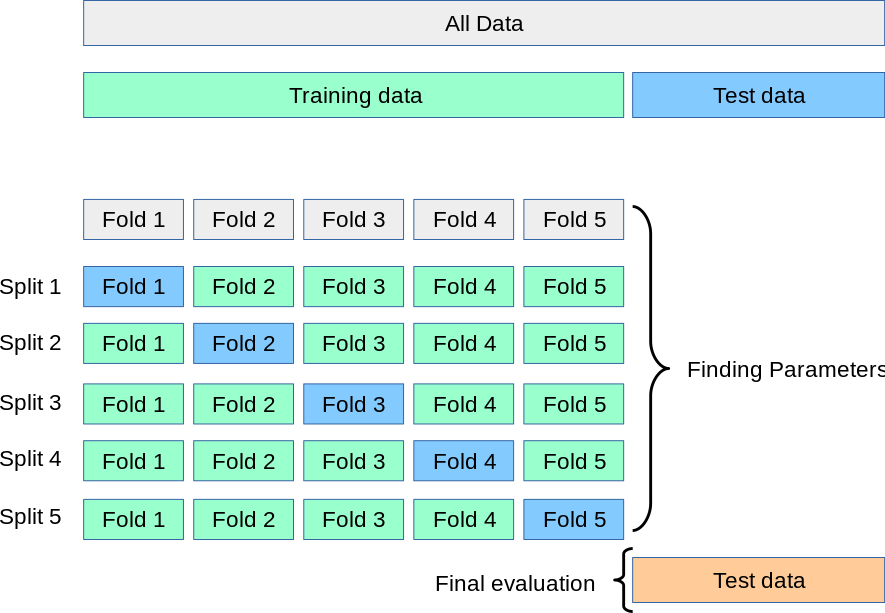
\includegraphics{../img/cross_validation.png}
\caption{scikit cross validation}
\end{figure}

Il motivo di tale suddivisione sono due: - aumentare il dataset
disponibile per train e test - offrire maggiore flessibilità e
generalizzazione

\hypertarget{proviamo-a-usare-scikit}{%
\subsection{Proviamo a usare scikit!}\label{proviamo-a-usare-scikit}}

Ora che abbiamo capito come funziona una regressione e come sia
possibile valutare tutto usando \href{https://scikit-learn.org/stable/index.html}{scikit}.

    \begin{tcolorbox}[breakable, size=fbox, boxrule=1pt, pad at break*=1mm,colback=cellbackground, colframe=cellborder]
\prompt{In}{incolor}{1}{\boxspacing}
\begin{Verbatim}[commandchars=\\\{\}]
\PY{k+kn}{import} \PY{n+nn}{pandas} \PY{k}{as} \PY{n+nn}{pd}
\PY{k+kn}{import} \PY{n+nn}{numpy} \PY{k}{as} \PY{n+nn}{np}
\PY{k+kn}{from} \PY{n+nn}{sklearn}\PY{n+nn}{.}\PY{n+nn}{datasets} \PY{k+kn}{import} \PY{n}{load\PYZus{}boston}

\PY{c+c1}{\PYZsh{}otteniamo il dataset}
\PY{n}{data} \PY{o}{=} \PY{n}{load\PYZus{}boston}\PY{p}{(}\PY{p}{)}
\PY{c+c1}{\PYZsh{}convertiamo il dataset in pandas}
\PY{n}{df} \PY{o}{=} \PY{n}{pd}\PY{o}{.}\PY{n}{DataFrame}\PY{p}{(}\PY{n}{data}\PY{o}{.}\PY{n}{data}\PY{p}{,} \PY{n}{columns} \PY{o}{=} \PY{n}{data}\PY{o}{.}\PY{n}{feature\PYZus{}names}\PY{p}{)}
\PY{n}{df}\PY{p}{[}\PY{l+s+s1}{\PYZsq{}}\PY{l+s+s1}{MEDV}\PY{l+s+s1}{\PYZsq{}}\PY{p}{]} \PY{o}{=} \PY{n}{data}\PY{o}{.}\PY{n}{target}
\PY{n}{display}\PY{p}{(}\PY{n}{df}\PY{p}{)}
\end{Verbatim}
\end{tcolorbox}

    
    \begin{Verbatim}[commandchars=\\\{\}]
        CRIM    ZN  INDUS  CHAS    NOX     RM   AGE     DIS  RAD    TAX  \textbackslash{}
0    0.00632  18.0   2.31   0.0  0.538  6.575  65.2  4.0900  1.0  296.0   
1    0.02731   0.0   7.07   0.0  0.469  6.421  78.9  4.9671  2.0  242.0   
2    0.02729   0.0   7.07   0.0  0.469  7.185  61.1  4.9671  2.0  242.0   
3    0.03237   0.0   2.18   0.0  0.458  6.998  45.8  6.0622  3.0  222.0   
4    0.06905   0.0   2.18   0.0  0.458  7.147  54.2  6.0622  3.0  222.0   
..       {\ldots}   {\ldots}    {\ldots}   {\ldots}    {\ldots}    {\ldots}   {\ldots}     {\ldots}  {\ldots}    {\ldots}   
501  0.06263   0.0  11.93   0.0  0.573  6.593  69.1  2.4786  1.0  273.0   
502  0.04527   0.0  11.93   0.0  0.573  6.120  76.7  2.2875  1.0  273.0   
503  0.06076   0.0  11.93   0.0  0.573  6.976  91.0  2.1675  1.0  273.0   
504  0.10959   0.0  11.93   0.0  0.573  6.794  89.3  2.3889  1.0  273.0   
505  0.04741   0.0  11.93   0.0  0.573  6.030  80.8  2.5050  1.0  273.0   

     PTRATIO       B  LSTAT  MEDV  
0       15.3  396.90   4.98  24.0  
1       17.8  396.90   9.14  21.6  
2       17.8  392.83   4.03  34.7  
3       18.7  394.63   2.94  33.4  
4       18.7  396.90   5.33  36.2  
..       {\ldots}     {\ldots}    {\ldots}   {\ldots}  
501     21.0  391.99   9.67  22.4  
502     21.0  396.90   9.08  20.6  
503     21.0  396.90   5.64  23.9  
504     21.0  393.45   6.48  22.0  
505     21.0  396.90   7.88  11.9  

[506 rows x 14 columns]
    \end{Verbatim}

    
    \hypertarget{usare-la-regressione-lineare-con-il-metrodo-olsordinary-least-square}{%
\subsubsection{Usare la regressione lineare con il metrodo OLS(Ordinary
Least
Square)}\label{usare-la-regressione-lineare-con-il-metrodo-olsordinary-least-square}}

Prima di vedere come applicare la regressione lineare, cerchiamo di
capire su cosa si basa il \textbf{metodo OLS} o chiamato anche in
italiano \textbf{metodo dei minimi quadrati}, la formula su cui si basa
il metodo è : \(\min_{w} \parallel wX - Y \parallel^2\). La formula
precedente ci dice che poiché noi possiamo controllare solo i valori di
\(w\), noi cerchiamo quei valori per cui la funzione assume il valore
minimo possibile, come vedremo in seguito questa funzione può portare a
problemi di \textbf{overfitting} o \textbf{underfitting} in particolare
quando utilizziamo il metodo del gradiente, vedremo poi in seguito delle
tecniche per ridurre questa possibiltà. Ora che abbiamo capito che
abbiamo un dataset con 506 dati e 13 colonne dette anche
\textbf{feature} e come funziona il metodo di regressione lineare,
proviamo a vedere il comportamento del Median value of owner-occupied
homes ogni 1000 dollari(MEDV) in funzione della lower status of the
population(LSTAT) e vediamo se facendo una regressione lineare cosa si
ottiene.

    \begin{tcolorbox}[breakable, size=fbox, boxrule=1pt, pad at break*=1mm,colback=cellbackground, colframe=cellborder]
\prompt{In}{incolor}{2}{\boxspacing}
\begin{Verbatim}[commandchars=\\\{\}]
\PY{k+kn}{import} \PY{n+nn}{plotly}\PY{n+nn}{.}\PY{n+nn}{graph\PYZus{}objects} \PY{k}{as} \PY{n+nn}{go}
\PY{k+kn}{from} \PY{n+nn}{sklearn}\PY{n+nn}{.}\PY{n+nn}{linear\PYZus{}model} \PY{k+kn}{import} \PY{n}{LinearRegression}
\PY{k+kn}{from} \PY{n+nn}{sklearn}\PY{n+nn}{.}\PY{n+nn}{model\PYZus{}selection} \PY{k+kn}{import} \PY{n}{train\PYZus{}test\PYZus{}split}

\PY{c+c1}{\PYZsh{}dividiamo il dataset in train e test}
\PY{n}{X\PYZus{}train}\PY{p}{,} \PY{n}{X\PYZus{}test}\PY{p}{,} \PY{n}{y\PYZus{}train}\PY{p}{,} \PY{n}{y\PYZus{}test} \PY{o}{=} \PY{n}{train\PYZus{}test\PYZus{}split}\PY{p}{(}\PY{n}{df}\PY{o}{.}\PY{n}{LSTAT}\PY{o}{.}\PY{n}{values}\PY{p}{,} \PY{n}{df}\PY{o}{.}\PY{n}{MEDV}\PY{o}{.}\PY{n}{values}\PY{p}{,} \PY{n}{random\PYZus{}state}\PY{o}{=}\PY{l+m+mi}{0}\PY{p}{,}
                                                   \PY{n}{test\PYZus{}size} \PY{o}{=} \PY{l+m+mf}{0.2}\PY{p}{)}

\PY{c+c1}{\PYZsh{}creiamo il modello con scikit}
\PY{n}{model} \PY{o}{=} \PY{n}{LinearRegression}\PY{p}{(}\PY{p}{)}
\PY{c+c1}{\PYZsh{}alleniamo il modello}
\PY{c+c1}{\PYZsh{}reshape (\PYZhy{}1,1) significa convertire i dati prima in array e poi come una matrice colonna}
\PY{n}{model}\PY{o}{.}\PY{n}{fit}\PY{p}{(}\PY{n}{X\PYZus{}train}\PY{o}{.}\PY{n}{reshape}\PY{p}{(}\PY{o}{\PYZhy{}}\PY{l+m+mi}{1}\PY{p}{,} \PY{l+m+mi}{1}\PY{p}{)}\PY{p}{,} \PY{n}{y\PYZus{}train}\PY{p}{)}

\PY{c+c1}{\PYZsh{}creiamo i futuri fit usando dei range}
\PY{n}{x\PYZus{}range} \PY{o}{=} \PY{n}{np}\PY{o}{.}\PY{n}{linspace}\PY{p}{(}\PY{n}{df}\PY{o}{.}\PY{n}{LSTAT}\PY{o}{.}\PY{n}{min}\PY{p}{(}\PY{p}{)}\PY{p}{,} \PY{n}{df}\PY{o}{.}\PY{n}{LSTAT}\PY{o}{.}\PY{n}{max}\PY{p}{(}\PY{p}{)}\PY{p}{,} \PY{l+m+mi}{100}\PY{p}{)}
\PY{n}{y\PYZus{}range} \PY{o}{=} \PY{n}{model}\PY{o}{.}\PY{n}{predict}\PY{p}{(}\PY{n}{x\PYZus{}range}\PY{o}{.}\PY{n}{reshape}\PY{p}{(}\PY{o}{\PYZhy{}}\PY{l+m+mi}{1}\PY{p}{,} \PY{l+m+mi}{1}\PY{p}{)}\PY{p}{)}

\PY{c+c1}{\PYZsh{}creiamo la figura}
\PY{n}{fig} \PY{o}{=} \PY{n}{go}\PY{o}{.}\PY{n}{Figure}\PY{p}{(}\PY{p}{[}
    \PY{n}{go}\PY{o}{.}\PY{n}{Scatter}\PY{p}{(}\PY{n}{x}\PY{o}{=}\PY{n}{X\PYZus{}train}\PY{p}{,} \PY{n}{y}\PY{o}{=}\PY{n}{y\PYZus{}train}\PY{p}{,} \PY{n}{name}\PY{o}{=}\PY{l+s+s1}{\PYZsq{}}\PY{l+s+s1}{train}\PY{l+s+s1}{\PYZsq{}}\PY{p}{,} \PY{n}{mode}\PY{o}{=}\PY{l+s+s1}{\PYZsq{}}\PY{l+s+s1}{markers}\PY{l+s+s1}{\PYZsq{}}\PY{p}{)}\PY{p}{,}
    \PY{n}{go}\PY{o}{.}\PY{n}{Scatter}\PY{p}{(}\PY{n}{x}\PY{o}{=}\PY{n}{X\PYZus{}test}\PY{p}{,}  \PY{n}{y}\PY{o}{=}\PY{n}{y\PYZus{}test}\PY{p}{,} \PY{n}{name}\PY{o}{=}\PY{l+s+s1}{\PYZsq{}}\PY{l+s+s1}{test}\PY{l+s+s1}{\PYZsq{}}\PY{p}{,} \PY{n}{mode}\PY{o}{=}\PY{l+s+s1}{\PYZsq{}}\PY{l+s+s1}{markers}\PY{l+s+s1}{\PYZsq{}}\PY{p}{)}\PY{p}{,}
    \PY{n}{go}\PY{o}{.}\PY{n}{Scatter}\PY{p}{(}\PY{n}{x}\PY{o}{=}\PY{n}{x\PYZus{}range}\PY{p}{,} \PY{n}{y}\PY{o}{=}\PY{n}{y\PYZus{}range}\PY{p}{,} \PY{n}{name}\PY{o}{=}\PY{l+s+s1}{\PYZsq{}}\PY{l+s+s1}{prediction}\PY{l+s+s1}{\PYZsq{}}\PY{p}{)}
\PY{p}{]}\PY{p}{)}
\PY{n}{fig}\PY{o}{.}\PY{n}{update\PYZus{}xaxes}\PY{p}{(}\PY{n}{title\PYZus{}text} \PY{o}{=} \PY{l+s+s2}{\PYZdq{}}\PY{l+s+s2}{LSTAT}\PY{l+s+s2}{\PYZdq{}}\PY{p}{)}
\PY{n}{fig}\PY{o}{.}\PY{n}{update\PYZus{}yaxes}\PY{p}{(}\PY{n}{title\PYZus{}text} \PY{o}{=} \PY{l+s+s2}{\PYZdq{}}\PY{l+s+s2}{MEDV}\PY{l+s+s2}{\PYZdq{}}\PY{p}{)}
\PY{n}{fig}\PY{o}{.}\PY{n}{show}\PY{p}{(}\PY{p}{)}
\end{Verbatim}
\end{tcolorbox}

    
    
    \begin{center}
    \adjustimage{max size={0.9\linewidth}{0.9\paperheight}}{output_3_1.png}
    \end{center}
    { \hspace*{\fill} \\}
    
    Per sapere come sia fatto il modello possiamo richiedere più
informazioni semplicemente richiamando le funzioni.

    \begin{tcolorbox}[breakable, size=fbox, boxrule=1pt, pad at break*=1mm,colback=cellbackground, colframe=cellborder]
\prompt{In}{incolor}{3}{\boxspacing}
\begin{Verbatim}[commandchars=\\\{\}]
\PY{n+nb}{print}\PY{p}{(}\PY{l+s+s1}{\PYZsq{}}\PY{l+s+s1}{Coefficienti modello}\PY{l+s+s1}{\PYZsq{}}\PY{p}{,} \PY{n}{model}\PY{o}{.}\PY{n}{coef\PYZus{}}\PY{p}{)}
\PY{n+nb}{print}\PY{p}{(}\PY{l+s+s1}{\PYZsq{}}\PY{l+s+s1}{Parametri}\PY{l+s+s1}{\PYZsq{}}\PY{p}{,} \PY{n}{model}\PY{o}{.}\PY{n}{get\PYZus{}params}\PY{p}{(}\PY{p}{)}\PY{p}{)}
\end{Verbatim}
\end{tcolorbox}

    \begin{Verbatim}[commandchars=\\\{\}]
Coefficienti modello [-0.95648761]
Parametri \{'copy\_X': True, 'fit\_intercept': True, 'n\_jobs': None, 'normalize':
False, 'positive': False\}
    \end{Verbatim}

    Per valutare come sia il uo score possiamo usare la funzione all'interno
dell'oggetto oppure usare delle metriche fornite da scikit.

    \begin{tcolorbox}[breakable, size=fbox, boxrule=1pt, pad at break*=1mm,colback=cellbackground, colframe=cellborder]
\prompt{In}{incolor}{4}{\boxspacing}
\begin{Verbatim}[commandchars=\\\{\}]
\PY{k+kn}{from} \PY{n+nn}{sklearn}\PY{n+nn}{.}\PY{n+nn}{metrics} \PY{k+kn}{import} \PY{n}{mean\PYZus{}absolute\PYZus{}error}\PY{p}{,} \PY{n}{mean\PYZus{}squared\PYZus{}error}\PY{p}{,} \PY{n}{r2\PYZus{}score}

\PY{c+c1}{\PYZsh{}create the predicted output}
\PY{n}{y\PYZus{}ptrain} \PY{o}{=} \PY{n}{model}\PY{o}{.}\PY{n}{predict}\PY{p}{(}\PY{n}{X\PYZus{}train}\PY{o}{.}\PY{n}{reshape}\PY{p}{(}\PY{o}{\PYZhy{}}\PY{l+m+mi}{1}\PY{p}{,} \PY{l+m+mi}{1}\PY{p}{)}\PY{p}{)}
\PY{n}{y\PYZus{}ptest}  \PY{o}{=} \PY{n}{model}\PY{o}{.}\PY{n}{predict}\PY{p}{(}\PY{n}{X\PYZus{}test}\PY{o}{.}\PY{n}{reshape}\PY{p}{(}\PY{o}{\PYZhy{}}\PY{l+m+mi}{1}\PY{p}{,} \PY{l+m+mi}{1}\PY{p}{)}\PY{p}{)}

\PY{n+nb}{print}\PY{p}{(}\PY{l+s+s1}{\PYZsq{}}\PY{l+s+s1}{R2 score}\PY{l+s+s1}{\PYZsq{}}\PY{p}{)}
\PY{n+nb}{print}\PY{p}{(}\PY{l+s+s1}{\PYZsq{}}\PY{l+s+s1}{Training Set:}\PY{l+s+s1}{\PYZsq{}}\PY{p}{,} \PY{n}{r2\PYZus{}score}\PY{p}{(}\PY{n}{X\PYZus{}train}\PY{p}{,}\PY{n}{y\PYZus{}ptrain}\PY{p}{)}\PY{p}{,} \PY{l+s+s1}{\PYZsq{}}\PY{l+s+s1}{Test Set:}\PY{l+s+s1}{\PYZsq{}}\PY{p}{,} \PY{n}{r2\PYZus{}score}\PY{p}{(}\PY{n}{X\PYZus{}test}\PY{p}{,} \PY{n}{y\PYZus{}ptest}\PY{p}{)}\PY{p}{)}
\PY{n+nb}{print}\PY{p}{(}\PY{l+s+s1}{\PYZsq{}}\PY{l+s+s1}{RMSE}\PY{l+s+s1}{\PYZsq{}}\PY{p}{)}
\PY{n+nb}{print}\PY{p}{(}\PY{l+s+s1}{\PYZsq{}}\PY{l+s+s1}{Training Set:}\PY{l+s+s1}{\PYZsq{}}\PY{p}{,} \PY{n}{mean\PYZus{}squared\PYZus{}error}\PY{p}{(}\PY{n}{X\PYZus{}train}\PY{p}{,}\PY{n}{y\PYZus{}ptrain}\PY{p}{)}\PY{p}{,} \PY{l+s+s1}{\PYZsq{}}\PY{l+s+s1}{Test Set:}\PY{l+s+s1}{\PYZsq{}}\PY{p}{,} \PY{n}{mean\PYZus{}squared\PYZus{}error}\PY{p}{(}\PY{n}{X\PYZus{}test}\PY{p}{,} \PY{n}{y\PYZus{}ptest}\PY{p}{)}\PY{p}{)}
\PY{n+nb}{print}\PY{p}{(}\PY{l+s+s1}{\PYZsq{}}\PY{l+s+s1}{MAE}\PY{l+s+s1}{\PYZsq{}}\PY{p}{)}
\PY{n+nb}{print}\PY{p}{(}\PY{l+s+s1}{\PYZsq{}}\PY{l+s+s1}{Training Set:}\PY{l+s+s1}{\PYZsq{}}\PY{p}{,} \PY{n}{mean\PYZus{}absolute\PYZus{}error}\PY{p}{(}\PY{n}{X\PYZus{}train}\PY{p}{,}\PY{n}{y\PYZus{}ptrain}\PY{p}{)}\PY{p}{,} \PY{l+s+s1}{\PYZsq{}}\PY{l+s+s1}{Test Set:}\PY{l+s+s1}{\PYZsq{}}\PY{p}{,} \PY{n}{mean\PYZus{}absolute\PYZus{}error}\PY{p}{(}\PY{n}{X\PYZus{}test}\PY{p}{,} \PY{n}{y\PYZus{}ptest}\PY{p}{)}\PY{p}{)}
\end{Verbatim}
\end{tcolorbox}

    \begin{Verbatim}[commandchars=\\\{\}]
R2 score
Training Set: -4.6742007815061575 Test Set: -5.418161658507217
RMSE
Training Set: 301.5495989395749 Test Set: 269.0927779444686
MAE
Training Set: 15.019429187947798 Test Set: 13.961546682555158
    \end{Verbatim}

    Ora che abbiamo capito come funziona il modello di scikit e come
possiamo testare e allenare su una serie di dati, proviamo ad applicare
il concetto di \textbf{cross validation}, per farlo utilizziamo la
funzione già presente in scikit e usiamo un numero di folds uguale a 5
applicando in ognuno il modello e vediamo cosa otteniamo.

    \begin{tcolorbox}[breakable, size=fbox, boxrule=1pt, pad at break*=1mm,colback=cellbackground, colframe=cellborder]
\prompt{In}{incolor}{5}{\boxspacing}
\begin{Verbatim}[commandchars=\\\{\}]
\PY{k+kn}{from} \PY{n+nn}{sklearn}\PY{n+nn}{.}\PY{n+nn}{model\PYZus{}selection} \PY{k+kn}{import} \PY{n}{cross\PYZus{}validate}

\PY{c+c1}{\PYZsh{}effettua la cross validation impostando il numero di folds e le metriche}
\PY{n}{cv\PYZus{}results} \PY{o}{=} \PY{n}{cross\PYZus{}validate}\PY{p}{(}\PY{n}{model}\PY{p}{,} \PY{n}{df}\PY{o}{.}\PY{n}{LSTAT}\PY{o}{.}\PY{n}{values}\PY{o}{.}\PY{n}{reshape}\PY{p}{(}\PY{o}{\PYZhy{}}\PY{l+m+mi}{1}\PY{p}{,}\PY{l+m+mi}{1}\PY{p}{)}\PY{p}{,} \PY{n}{df}\PY{o}{.}\PY{n}{MEDV}\PY{o}{.}\PY{n}{values}\PY{p}{,} \PY{n}{cv} \PY{o}{=}\PY{l+m+mi}{5}\PY{p}{,}
                            \PY{n}{scoring} \PY{o}{=} \PY{p}{[}\PY{l+s+s1}{\PYZsq{}}\PY{l+s+s1}{r2}\PY{l+s+s1}{\PYZsq{}}\PY{p}{,} \PY{l+s+s1}{\PYZsq{}}\PY{l+s+s1}{neg\PYZus{}mean\PYZus{}squared\PYZus{}error}\PY{l+s+s1}{\PYZsq{}}\PY{p}{,} \PY{l+s+s1}{\PYZsq{}}\PY{l+s+s1}{neg\PYZus{}mean\PYZus{}absolute\PYZus{}error}\PY{l+s+s1}{\PYZsq{}}\PY{p}{]}\PY{p}{,}
                            \PY{n}{return\PYZus{}train\PYZus{}score} \PY{o}{=} \PY{k+kc}{True}\PY{p}{)}
\PY{n}{display}\PY{p}{(}\PY{n}{cv\PYZus{}results}\PY{p}{)}
\end{Verbatim}
\end{tcolorbox}

    
    \begin{Verbatim}[commandchars=\\\{\}]
\{'fit\_time': array([0.00100374, 0.00099945, 0.00100064, 0.00100541, 0.00100136]),
 'score\_time': array([0.0019958 , 0.00099945, 0.00100136, 0.00099874, 0.        ]),
 'test\_r2': array([0.31784807, 0.5406078 , 0.07608699, 0.42423767, 0.1267687 ]),
 'train\_r2': array([0.55953888, 0.53499276, 0.55004371, 0.5617624 , 0.5056059 ]),
 'test\_neg\_mean\_squared\_error': array([-23.55825   , -41.82157437, -73.99360893, -50.50118016,
        -23.21775049]),
 'train\_neg\_mean\_squared\_error': array([-42.7285291 , -37.97136234, -31.25967296, -35.78590001,
        -42.49238511]),
 'test\_neg\_mean\_absolute\_error': array([-4.18200738, -4.38425663, -6.00666715, -5.43917773, -3.74895682]),
 'train\_neg\_mean\_absolute\_error': array([-4.81563608, -4.39256578, -3.88848603, -4.44496347, -4.84370493])\}
    \end{Verbatim}

    
    I dati che abbiamo ottenuto rappresentano i valori di score del modello
usando le diverse metriche, come possiamo notare i valori in genere sono
in simili sia in fase di training e di testing, questo significa che il
modello è in grado di generalizzare indipendentemente dalla sezione del
dataset che si usa per allenare. Qualora volessimo solo ottenere le
previsioni del modello senza considerare lo scoring possiamo usare un
altra funzione di scikit:

    \begin{tcolorbox}[breakable, size=fbox, boxrule=1pt, pad at break*=1mm,colback=cellbackground, colframe=cellborder]
\prompt{In}{incolor}{6}{\boxspacing}
\begin{Verbatim}[commandchars=\\\{\}]
\PY{k+kn}{from} \PY{n+nn}{sklearn}\PY{n+nn}{.}\PY{n+nn}{model\PYZus{}selection} \PY{k+kn}{import} \PY{n}{cross\PYZus{}val\PYZus{}predict}

\PY{n}{pred\PYZus{}results} \PY{o}{=} \PY{n}{cross\PYZus{}val\PYZus{}predict}\PY{p}{(}\PY{n}{model}\PY{p}{,} \PY{n}{df}\PY{o}{.}\PY{n}{LSTAT}\PY{o}{.}\PY{n}{values}\PY{o}{.}\PY{n}{reshape}\PY{p}{(}\PY{o}{\PYZhy{}}\PY{l+m+mi}{1}\PY{p}{,}\PY{l+m+mi}{1}\PY{p}{)}\PY{p}{,} \PY{n}{df}\PY{o}{.}\PY{n}{MEDV}\PY{o}{.}\PY{n}{values}\PY{p}{,} \PY{n}{cv} \PY{o}{=}\PY{l+m+mi}{5}\PY{p}{)}
\PY{n}{display}\PY{p}{(}\PY{n}{pred\PYZus{}results}\PY{p}{)}
\end{Verbatim}
\end{tcolorbox}

    
    \begin{Verbatim}[commandchars=\\\{\}]
array([30.70217411, 26.55374947, 31.6495307 , 32.73649774, 30.353148  ,
       30.4728141 , 23.27290401, 16.57160266,  5.8215984 , 18.61589846,
       15.27521996, 22.43524134, 20.00203073, 27.43130083, 25.43686591,
       27.22188517, 29.10662617, 21.03913689, 24.01084493, 24.41970409,
       14.706806  , 21.87679956, 17.00040617, 15.84363391, 19.41367243,
       19.20425676, 20.89952645, 18.43639931, 22.90393355, 23.72165187,
       13.13120241, 22.66460136,  8.03542117, 17.36937663, 15.38491388,
       26.01525204, 24.29006582, 26.92271993, 25.56650418, 31.36033764,
       33.6938265 , 30.84178456, 29.87448362, 28.24901915, 26.14489031,
       25.48672678, 21.55768997, 16.92062877,  4.94404704, 19.51339418,
       22.2557422 , 26.2645564 , 30.40300887, 27.26177386, 20.90949862,
       30.87170108, 29.91437232, 31.7293081 , 28.82740528, 26.47397207,
       22.55490744, 21.26849691, 28.95704355, 26.19475118, 27.6407165 ,
       31.01131153, 25.45681026, 27.59085563, 22.61474049, 26.90277558,
       28.96701573, 25.81580854, 30.16367668, 28.14929741, 28.90718268,
       26.75319296, 23.73162404, 25.42689373, 23.36265358, 26.59363816,
       30.3930367 , 28.46840699, 28.96701573, 28.17921393, 26.07508508,
       29.15648704, 22.8441005 , 27.25180169, 30.18362103, 29.98417754,
       26.88283123, 27.49113388, 27.53102258, 29.47559663, 25.10778414,
       29.03682095, 24.35987105, 31.47003156, 32.10825074, 29.49554098,
       26.27452858, 28.01965914, 23.93156342, 21.33844389, 22.36277224,
       18.54230433, 16.52133217, 20.73861197, 22.41814134, 19.3912972 ,
       21.74448396, 24.36528804, 18.78223709, 17.97015696, 24.09767072,
       19.19750535, 22.63038956, 24.23609347, 19.5574045 , 21.18156477,
       20.48022284, 20.57250467, 17.19498955, 10.29230839, 17.51797597,
       20.07418277,  8.58509446, 17.87787512, 19.53894813, 16.81663403,
       22.11361129, 22.42736953, 23.47938243, 19.87116273, 17.76713692,
       18.09012334, 18.14549244, 20.2772028 , 14.06663539, 16.70589583,
       11.44583131,  1.98694335,  8.99113453,  9.36026187,  6.71177324,
        8.08677256, 18.37619703,  6.49029684,  7.60690702, 13.946669  ,
       20.72938379, 21.48609482, 22.55656409, 19.1698208 , 19.78810908,
       19.88039092, 18.84683438, 29.50538618, 27.80740044, 26.92149483,
       28.66562149, 32.14464662, 31.96931114, 30.67736547, 22.9995169 ,
       24.68827445, 30.3266945 , 22.53810773, 23.4978388 , 23.29481876,
       20.42485373, 22.63961775, 20.18492097, 25.39884457, 24.84515357,
       28.82250061, 24.41142895, 27.936595  , 27.35521945, 29.09011793,
       26.76461571, 25.02048906, 29.29313796, 28.49951419, 20.84012199,
       21.60606121, 29.63458074, 27.57669585, 29.53307073, 28.76713151,
       29.03474883, 29.41310434, 31.09263372, 29.09934611, 29.69917803,
       31.00035188, 29.97602353, 25.79565646, 27.63206495, 29.53307073,
       29.63458074, 26.8845821 , 30.87115732, 29.17668809, 29.97268057,
       23.13399246, 23.04840187, 16.98002907, 19.89010911, 12.67482241,
       17.65619472, 11.91306616, 18.71751804, 24.40929225,  7.14567032,
       24.33226072, 20.87440089, 24.14396142, 17.09985589, 23.45067764,
       24.1268433 , 14.06994902, 23.938544  , 25.93280474, 28.89423914,
       28.47484525, 29.7587041 , 26.99412805, 29.08253844, 29.21948338,
       22.46638586, 27.9441836 , 30.32360199, 29.05686126, 25.54764709,
       23.1254334 , 24.2723473 , 28.38925466, 26.99412805, 26.1296631 ,
       22.69748045, 21.82445644, 22.8344254 , 27.99553795, 21.73886585,
       16.63766671, 24.59759154, 23.75024471, 24.28946542, 26.82294687,
       27.38784477, 29.36498739, 29.41634174, 29.40778268, 26.81438782,
       24.52056001, 29.77582222, 28.05545137, 25.77018262, 26.53193887,
       24.22955201, 26.22381275, 27.37928571, 22.80874822, 25.50485179,
       23.49347294, 19.77884135, 26.06974969, 29.73302692, 20.75457407,
       21.3109129 , 26.7972697 , 25.82153698, 26.80582876, 29.41634174,
       29.88708998, 27.25945888, 28.87712103, 26.28372616, 28.28654596,
       29.21948338, 28.50908149, 29.86141281, 29.73302692, 25.71882827,
       25.39358403, 21.37082631, 26.32652145, 25.93280474, 24.29802448,
       29.58752292, 29.39066456, 28.41493184, 25.09401696, 23.53626823,
       27.07115958, 26.11254498, 18.88014016, 28.18383725, 28.38069561,
       27.24234076, 24.30658354, 25.01698543, 28.2779869 , 28.59823713,
       26.61343853, 29.05474081, 28.00279755, 30.97007147, 25.58134325,
       22.93163711, 29.54101647, 23.84464447, 27.63560981, 26.26609877,
       24.06297232, 17.28488508, 19.65671942, 25.19430753, 22.84232118,
       28.33028932, 28.65778109, 27.83408967, 23.82479649, 29.40208057,
       30.43417584, 29.37230859, 22.78277722, 25.58134325, 28.19135342,
       26.45465464, 23.14004097, 27.70507776, 29.83873626, 28.77686901,
       27.52644589, 25.75005114, 24.99582766, 27.03024624, 25.80959509,
       26.25617478, 30.02729213, 26.89131033, 28.35013731, 30.90060352,
       25.02559964, 22.90186514, 29.16390474, 29.53109248, 29.63033241,
       29.54101647, 30.02729213, 27.74477373, 31.00976744, 27.48674992,
       29.94790019, 18.00933657, 22.30642555, 24.08282031, 22.90186514,
       27.74477373, 21.3934182 , 25.36301541, 20.94683851, 30.22577199,
       28.40968127, 21.58197406, 22.2468816 , 32.24034258, 31.7739149 ,
       32.53806237, 26.01799895, 26.66305849,  0.96984054, -2.20583723,
       22.13771767, 12.4122045 , 14.39700311, 11.96562482, 13.86110749,
       18.3963723 , 14.555787  , 12.05494076, 11.10223742,  5.07837366,
        4.89974178,  7.41051202,  3.7287106 ,  5.08829765, 14.78403884,
       18.49561223, 16.85815338,  9.99075021, 20.42086688, 19.2498357 ,
       18.48568824, 16.25278981, 15.70697019,  5.11806963,  5.7333572 ,
        8.90903497, 15.31001047, 15.31993446, 15.85583009,  8.30367139,
       12.99231392, 12.64600977, 23.42953623,  9.70242449, 16.07057304,
       25.3726873 , 14.68535643,  2.03563538, 15.78198624, -0.47506971,
        7.15324116, 10.28921763,  9.47155506, 15.26253002, 13.22318335,
       20.64948347, 19.99535341, 21.53448296, 12.69410757, 18.59089769,
       11.635956  , 20.00497297, 21.13046146, 14.39676964, 11.93416235,
       18.12915882, 16.15714907, 23.52573183, 19.4951363 , 20.50519007,
       12.71334669, 17.73475687,  9.65432669,  2.37231997, 13.08850952,
       13.82921562, 16.32068159, 19.13921259, 16.96519209, 12.21312958,
       12.03035795, 17.98486542, 19.28350599, 17.65780039, 16.52269234,
       18.32155001, 18.04258278, 18.48508253, 18.99491919, 17.09986593,
       17.65780039, 16.81127913, 18.802528  , 19.48551674, 20.95730938,
       19.30274511, 21.00540718, 21.64029812, 25.19953522, 22.38100422,
       21.50562429, 18.60051725, 14.58916084, 17.65780039, 20.89959202,
       19.42779938, 22.71768881, 21.28437441, 23.88165554, 17.64818083,
       11.91492323, 17.12872461, 11.13573889, 17.75399599, 22.48681938,
       24.76665504, 27.65252296, 28.35475082, 25.07448095, 22.2655695 ,
       24.92056799, 20.68796171, 24.08366629, 17.72513731, 12.03997751,
        6.5472089 , 17.71551775, 22.25594994, 23.54497095, 22.02508051,
       18.16763706, 14.76231291, 21.53448296, 22.66959101, 20.57252699,
       21.31323309, 25.79594793, 26.36350195, 29.6726305 , 28.86458748,
       27.51784912])
    \end{Verbatim}

    
    \hypertarget{multiple-linear-regression-mlr}{%
\subsection{Multiple Linear Regression
(MLR)}\label{multiple-linear-regression-mlr}}

Nel caso in cui si abbia un dataset che contiene molte features è
possibile usare una \textbf{MLR} ovvero una regressione lineare su più
variabili indipendenti per la previsione di una variabile dipendente da
tutte quelle impostate nel modello, vediamo in dettaglio come usarlo.

    \begin{tcolorbox}[breakable, size=fbox, boxrule=1pt, pad at break*=1mm,colback=cellbackground, colframe=cellborder]
\prompt{In}{incolor}{7}{\boxspacing}
\begin{Verbatim}[commandchars=\\\{\}]
\PY{c+c1}{\PYZsh{}prendiamo ogni colonna tranne quella di MEDV}
\PY{n}{X} \PY{o}{=} \PY{n}{df}\PY{o}{.}\PY{n}{drop}\PY{p}{(}\PY{l+s+s1}{\PYZsq{}}\PY{l+s+s1}{MEDV}\PY{l+s+s1}{\PYZsq{}}\PY{p}{,} \PY{n}{axis} \PY{o}{=} \PY{l+m+mi}{1}\PY{p}{)}
\PY{n}{Y} \PY{o}{=} \PY{n}{df}\PY{p}{[}\PY{p}{[}\PY{l+s+s1}{\PYZsq{}}\PY{l+s+s1}{MEDV}\PY{l+s+s1}{\PYZsq{}}\PY{p}{]}\PY{p}{]}
\PY{c+c1}{\PYZsh{}aplichiamo il modello ora non più in un contesto 1D }
\PY{c+c1}{\PYZsh{}effettua la cross validation impostando il numero di folds e le metriche}
\PY{n}{cv\PYZus{}results} \PY{o}{=} \PY{n}{cross\PYZus{}validate}\PY{p}{(}\PY{n}{model}\PY{p}{,} \PY{n}{X}\PY{p}{,} \PY{n}{Y}\PY{p}{,} \PY{n}{cv} \PY{o}{=}\PY{l+m+mi}{5}\PY{p}{,}
                            \PY{n}{scoring} \PY{o}{=} \PY{p}{[}\PY{l+s+s1}{\PYZsq{}}\PY{l+s+s1}{r2}\PY{l+s+s1}{\PYZsq{}}\PY{p}{,} \PY{l+s+s1}{\PYZsq{}}\PY{l+s+s1}{neg\PYZus{}mean\PYZus{}squared\PYZus{}error}\PY{l+s+s1}{\PYZsq{}}\PY{p}{,} \PY{l+s+s1}{\PYZsq{}}\PY{l+s+s1}{neg\PYZus{}mean\PYZus{}absolute\PYZus{}error}\PY{l+s+s1}{\PYZsq{}}\PY{p}{]}\PY{p}{,}
                            \PY{n}{return\PYZus{}train\PYZus{}score} \PY{o}{=} \PY{k+kc}{True}\PY{p}{)}
\PY{n}{display}\PY{p}{(}\PY{n}{cv\PYZus{}results}\PY{p}{)}
\end{Verbatim}
\end{tcolorbox}

    
    \begin{Verbatim}[commandchars=\\\{\}]
\{'fit\_time': array([0.00599957, 0.00400114, 0.00400162, 0.00500011, 0.00600934]),
 'score\_time': array([0.00700021, 0.00699854, 0.00600004, 0.00599885, 0.00698924]),
 'test\_r2': array([ 0.63919994,  0.71386698,  0.58702344,  0.07923081, -0.25294154]),
 'train\_r2': array([0.74652533, 0.72763185, 0.69498059, 0.84181027, 0.73545537]),
 'test\_neg\_mean\_squared\_error': array([-12.46030057, -26.04862111, -33.07413798, -80.76237112,
        -33.31360656]),
 'train\_neg\_mean\_squared\_error': array([-24.5892302 , -22.24092194, -21.19051839, -12.91756328,
        -22.73718934]),
 'test\_neg\_mean\_absolute\_error': array([-2.62190565, -3.90725478, -4.386606  , -5.57073637, -4.76333993]),
 'train\_neg\_mean\_absolute\_error': array([-3.55584094, -3.29666359, -3.20481356, -2.74360523, -3.30689921])\}
    \end{Verbatim}

    
    \begin{center}\rule{0.5\linewidth}{0.5pt}\end{center}

A PRESTO, SPERIAMO CHE QUESTA LEZIONE SIA STATA PIACEVOLE!


    % Add a bibliography block to the postdoc
    
    
    
\end{document}
